 The following definition modifies~\cite[\textdef~5.9]{endrullis2024generalized}.
\begin{definition}[Decreasing Rules]
    \label{def:decreasing_rule}
    Let $\mathcal{T} = (T,\mathbb{E}, (S, \oplus, \odot, 0_S, 1_S, \prec, \mu), w)$ be a finitary weighted type graph, \(\mathfrak{F}\) a DPO rewriting framework, $\rho = (L \overset{l}{\leftarrow} K \overset{r}{\rightarrow} R)$ a DPO rewriting rule, and $\delta \in \mathbb{R}_{>0}$. 

    \noindent
    The rule $\rho$ is \textbf{weakly decreasing} w.r.t. $\mathcal{T}$ in $\mathfrak{F}$ if 
            for every $t_K : K \to T$,
                $$ 
                  w_\mathcal{T}(\{l \star - = t_K\}) \succeq w_\mathcal{T}(\{r\star - = t_K\})$$
           
    \noindent
    The rule $\rho$ is \textbf{$\delta$-uniformly decreasing} w.r.t. $\mathcal{T}$ in $\mathfrak{F}$ if the following hold:
        \begin{itemize}
            \item[]- there exists a context closure $c_\rho$ for $\rho$ and $\mathcal{T}$ in $\mathfrak{F}$, 
            \item[]- for every $t_K : K \to T$,
            \begin{itemize}
                \item[] $\bullet$ $\{l \star - = t_K\} = \emptyset = \{r \star - = t_K\}$, or
                \item[] $\bullet$ $\mu(w_\mathcal{T}(\{l \star - = t_K\}))  >   \mu(w_\mathcal{T}(\{r \star - = t_K\})) + \delta$.
            \end{itemize}
        \end{itemize}  
         
    \noindent
    The rule $\rho$ is
            \textbf{$\delta$-closure decreasing} w.r.t. $\mathcal{T}$ in $\mathfrak{F}$ if the following hold:
            \begin{itemize}
                \item[]- $S$ is strictly monotonic measurable semiring,
                \item[]- $\rho$ is weakly decreasing,
                \item[]- there exists a context closure $c_\rho$ for $\rho$ and $\mathcal{T}$ in $\mathfrak{F}$,
                \item[]- $ \mu(w_\mathcal{T}(\{l \star - = t_K\}))  >  \mu(w_\mathcal{T}(\{r \star - = t_K\}))  + \delta$ for $t_K = l \star c_\rho$.
            \end{itemize}
\end{definition}

\begin{example}
    \label{example:decreasing_rule}
    Consider the DPO rule in Example~\ref{ex:grsaa} and the weighted type graph in~\autoref{example:weighted_type_graph} over the real arithmetic semiring $\mathfrak{N}' = (\mathbb{R}^+,+,*,0_\mathbb{R},1_\mathbb{R},<,\operatorname{id}_{\mathbb{R}^+})$. There are $t_K^{11}, t_K^{12}, t_K^{21}, t_K^{22}:K \rightarrow T$ as depicted below:

    \begin{center}
        \resizebox{0.49\textwidth}{!}{
            \begin{tikzpicture}
            \graphbox{\( K \)}{-50mm}{0mm}{40mm}{30mm}{2mm}{-6mm}{
                \coordinate (o) at (0mm,-10mm); 
                \node[draw,circle] (l1) at ($(o)+(-10mm,0mm)$) {1};
                \node[draw,circle] (l2) at ($(l1)+(2,0)$) {2};
                % \node[draw,circle] (l3) at ($(l1) + (1,0)$) {3};
                % \draw[] (l1) -- (l3) node[midway,above] {$a$};
                % \draw[] (l3) -- (l2) node[midway,above] {$a$};
            } 
                \graphbox{$T$}{0mm}{0mm}{40mm}{30mm}{-10mm}{-15mm}{
                    \node[draw,circle] (1) at (0,0) {$1\ 2$};
                    \node[draw,circle] (2) at (2,0) {};
                    \draw[->] (1) edge[loop above] node[midway, above] {$a$} (1) ;
                    \draw[->] (1) edge[loop below] node[midway, below] {$b$} (1) ;
                    \draw[->] (1) edge[bend left] node[midway, above] {$a$}  (2)  ;
                    \draw[->] (2) edge[bend left] node[midway, below] {$a$} (1)   ;
                }
                \node () at (-5mm,-15mm) {$\overset{t_K^{11}}{\to}$};
            \end{tikzpicture}
            } 
            \resizebox{0.49\textwidth}{!}{
            \begin{tikzpicture}
                \graphbox{\( K \)}{-50mm}{0mm}{40mm}{30mm}{2mm}{-6mm}{
                \coordinate (o) at (0mm,-10mm); 
                \node[draw,circle] (l1) at ($(o)+(-10mm,0mm)$) {1};
                \node[draw,circle] (l2) at ($(l1)+(2,0)$) {2};
                % \node[draw,circle] (l3) at ($(l1) + (1,0)$) {3};
                % \draw[] (l1) -- (l3) node[midway,above] {$a$};
                % \draw[] (l3) -- (l2) node[midway,above] {$a$};
            } 
                \graphbox{$T$}{0mm}{0mm}{40mm}{30mm}{-10mm}{-15mm}{
                    \node[draw,circle] (1) at (0,0) {$1$};
                    \node[draw,circle] (2) at (2,0) {2};
                    \draw[->] (1) edge[loop above] node[midway, above] {$a$} (1) ;
                    \draw[->] (1) edge[loop below] node[midway, below] {$b$} (1) ;
                    \draw[->] (1) edge[bend left] node[midway, above] {$a$}  (2)  ;
                    \draw[->] (2) edge[bend left] node[midway, below] {$a$} (1)   ;
                }
                \node () at (-5mm,-15mm) {$\overset{t_K^{12}}{\to}$};
            \end{tikzpicture}
            }
            \resizebox{0.49\textwidth}{!}{
            \begin{tikzpicture}
                \graphbox{\( K \)}{-50mm}{0mm}{40mm}{30mm}{2mm}{-6mm}{
                \coordinate (o) at (0mm,-10mm); 
                \node[draw,circle] (l1) at ($(o)+(-10mm,0mm)$) {1};
                \node[draw,circle] (l2) at ($(l1)+(2,0)$) {2};
                % \node[draw,circle] (l3) at ($(l1) + (1,0)$) {3};
                % \draw[] (l1) -- (l3) node[midway,above] {$a$};
                % \draw[] (l3) -- (l2) node[midway,above] {$a$};
            } 
                \graphbox{$T$}{0mm}{0mm}{40mm}{30mm}{-10mm}{-15mm}{
                    \node[draw,circle] (1) at (0,0) {2};
                    \node[draw,circle] (2) at (2,0) {1};
                    \draw[->] (1) edge[loop above] node[midway, above] {$a$} (1) ;
                    \draw[->] (1) edge[loop below] node[midway, below] {$b$} (1) ;
                    \draw[->] (1) edge[bend left] node[midway, above] {$a$}  (2)  ;
                    \draw[->] (2) edge[bend left] node[midway, below] {$a$} (1)   ;
                }
                \node () at (-5mm,-15mm) {$\overset{t_K^{21}}{\to}$};
            \end{tikzpicture}
            }
            \resizebox{0.49\textwidth}{!}{
            \begin{tikzpicture}
                \graphbox{\( K \)}{-50mm}{0mm}{40mm}{30mm}{2mm}{-6mm}{
                \coordinate (o) at (0mm,-10mm); 
                \node[draw,circle] (l1) at ($(o)+(-10mm,0mm)$) {1};
                \node[draw,circle] (l2) at ($(l1)+(2,0)$) {2};
                % \node[draw,circle] (l3) at ($(l1) + (1,0)$) {3};
                % \draw[] (l1) -- (l3) node[midway,above] {$a$};
                % \draw[] (l3) -- (l2) node[midway,above] {$a$};
            } 
                \graphbox{$T$}{0mm}{0mm}{40mm}{30mm}{-10mm}{-15mm}{
                    \node[draw,circle] (1) at (0,0) {};
                    \node[draw,circle] (2) at (2,0) {$1\ 2$};
                    \draw[->] (1) edge[loop above] node[midway, above] {$a$} (1) ;
                    \draw[->] (1) edge[loop below] node[midway, below] {$b$} (1) ;
                    \draw[->] (1) edge[bend left] node[midway, above] {$a$}  (2)  ;
                    \draw[->] (2) edge[bend left] node[midway, below] {$a$} (1)   ;
                }
                \node () at (-5mm,-15mm) {$\overset{t_K^{22}}{\to}$};
            \end{tikzpicture}
            }
      \end{center}
    The set $\{l \star - = t_K^{11}\}$ has two morphisms $h_{11}^1$ and $h_{11}^2$ as illustrated below:
    \begin{center}
        \resizebox{0.49\textwidth}{!}{
        \begin{tikzpicture}
          \graphbox{\( L \)}{-50mm}{0mm}{40mm}{35mm}{2mm}{-6mm}{
            \coordinate (o) at (0mm,-10mm); 
            \node[draw,circle] (l1) at ($(o)+(-10mm,0mm)$) {1};
            \node[draw,circle] (l2) at ($(l1)+(2,0)$) {2};
            \node[draw,circle] (l3) at ($(l1) + (1,0)$) {3};
            \draw[] (l1) -- (l3) node[midway,above] {$a$};
            \draw[] (l3) -- (l2) node[midway,above] {$a$};
        } 
            \graphbox{$T$}{0mm}{0mm}{40mm}{35mm}{-10mm}{-17mm}{
                \node[draw,circle] (1) at (0,0) {$1\ 2$};
                \node[draw,circle] (2) at (2,0) {3};
                \draw[->] (1) edge[loop above] node[midway, above] {$a^{1.0}$} (1) ;
                \draw[->] (1) edge[loop below] node[midway, below] {$b^{1.0}$} (1) ;
                \draw[->] (1) edge[bend left] node[midway, above] {$a^{1.0}$}  (2)  ;
                \draw[->] (2) edge[bend left] node[midway, below] {$a^{1.0}$} (1)   ;
            }
            \node () at (-5mm,-15mm) {$\overset{h_{11}^1}{\to}$};
        \end{tikzpicture}
        }
        \resizebox{0.49\textwidth}{!}{
            \begin{tikzpicture}
              \graphbox{\(L\)}{-50mm}{0mm}{40mm}{35mm}{2mm}{-6mm}{
                \coordinate (o) at (0mm,-10mm); 
                \node[draw,circle] (l1) at ($(o)+(-10mm,0mm)$) {1};
                \node[draw,circle] (l2) at ($(l1)+(2,0)$) {2};
                \node[draw,circle] (l3) at ($(l1) + (1,0)$) {3};
                \draw[] (l1) -- (l3) node[midway,above] {$a$};
                \draw[] (l3) -- (l2) node[midway,above] {$a$};
            } 
                \graphbox{$T$}{0mm}{0mm}{40mm}{35mm}{-10mm}{-17mm}{
                    \node[draw,circle] (1) at (0,0) {$1\ 2\ 3$};
                    \node[draw,circle] (2) at (2,0) {};
                    \draw[->] (1) edge[loop above] node[midway, above] {$a^{1.0}$} (1) ;
                    \draw[->] (1) edge[loop below] node[midway, below] {$b^{1.0}$} (1) ;
                    \draw[->] (1) edge[bend left] node[midway, above] {$a^{1.0}$}  (2)  ;
                    \draw[->] (2) edge[bend left] node[midway, below] {$a^{1.0}$} (1)   ;(1)   ;
                }
                \node () at (-5mm,-15mm) {$\overset{h_{11}^2}{\to}$};
            \end{tikzpicture}
            }
      \end{center}
    Therefore, we have \begin{flalign*}
        w_\mathcal{T}(\{l \star - = t_K^{11}\})
        =&w_\mathcal{T}(\{h_{11}^1, h_{11}^2\})\\
        \overset{\mathrm{def}}{=}&w_\mathcal{T}(h_{11}^1) + w_\mathcal{T}(h_{11}^2) \\
        =&(1.0^1 * 1.0^1) + (1.0^1 * 1.0^1)\\
        =&2.0
    \end{flalign*}
    The set $\{r \star - = t_K^{11}\}$ has one morphism $h_{11}^3$ as illustrated below:
    \begin{center}
        \resizebox{0.49\textwidth}{!}{
        \begin{tikzpicture}
          \graphbox{\( R \)}{-55mm}{0mm}{45mm}{40mm}{1mm}{-19mm}{
            \coordinate (o) at (-5mm,-3mm); 
            \node[draw,circle] (l1) at ($(o)+(-10mm,0mm)$) {1};
            \node[draw,circle] (l2) at ($(l1)+(3,0)$) {2};
            \node[draw,circle] (l3) at ($(l1) + (1,0)$) {4};
            \node[draw,circle] (l4) at ($(l1) + (2,0)$) {5};
            \draw[->] (l1) -- (l3) node[midway,above] {$a$};
            \draw[->] (l3) -- (l4) node[midway,above] {$b$};
            \draw[->] (l4) -- (l2) node[midway,above] {$a$};
        } 
            \graphbox{$T$}{0mm}{0mm}{40mm}{40mm}{-10mm}{-20mm}{
                \node[draw,circle] (1) at (0,0) {$1\ 2\ 4\ 5$};
                \node[draw,circle] (2) at (2,0) {};
                \draw[->] (1) edge[loop above] node[midway, above] {$a^{1.0}$} (1) ;
                \draw[->] (1) edge[loop below] node[midway, below] {$b^{1.0}$} (1) ;
                \draw[->] (1) edge[bend left] node[midway, above] {$a^{1.0}$}  (2)  ;
                \draw[->] (2) edge[bend left] node[midway, below] {$a^{1.0}$} (1)   ;
            }
            \node () at (-5mm,-19mm) {$\overset{h_{11}^1}{\to}$};
        \end{tikzpicture}
        }
      \end{center}
    Therefore, we have: $w_\mathcal{T}(\{r \star - = t_K^{11}\}) = w_\mathcal{T}(h_{11}^3) = 1.0^1 * 1.0^1 * 1.0 ^ 1 = 1.0$. Thus, we have $w_\mathcal{T}(\{l \star - = t_K^{11}\}) = 2.0 \geq 1.0 = w_\mathcal{T}(\{r \star - = t_K^{11}\})$.

    Similarly, we can check that $w_\mathcal{T}(\{l \star - = t_K^{12}\}) = 1.0 \geq 1.0 = w_\mathcal{T}(\{r \star - = t_K^{12}\})$,  $w_\mathcal{T}(\{l \star - = t_K^{21}\}) = 1.0 \geq 1.0 = w_\mathcal{T}(\{r \star - = t_K^{21}\})$, and $w_\mathcal{T}(\{l \star - = t_K^{22}\}) = 1.0 \geq 1.0 = w_\mathcal{T}(\{r \star - = t_K^{22}\})$. The rule is therefore weakly decreasing.

    There exists a context closure $c$ for the DPO rule in the weighted type graph, as shown in~\autoref{example:context_closure}.
    Since we have additionally $t_K^{11} = l \star c$ and $w_\mathcal{T}(\{l \star - = t_K^{11}\}) = 1.0 > 1.0 + \delta$ for $\delta = 1.0$, the rule is $\delta$-closure decreasing with $\delta = 1.0$ since the semiring is strictly monotonic measurable.

\end{example}

Adapted from \cite[Theorem C.3]{endrullis2024generalized}, the lemma below establishes that decreasing rules reduce the weights of host graphs, provided specific constraints are satisfied.
\begin{lemma}[Decreasing steps]
    \label{lem:decreasing_step}
\newline
\begin{minipage}{0.7\textwidth}
    Let $\mathcal{T} = (T,\mathbb{E}, (S, \oplus, \odot, 0_S, 1_S, \prec, \mu), w)$ be a finitary weighted type graph, $\rho$ a rewriting rule and $\Delta \in \mathfrak{F}(\rho)$ a DPO diagram
    (shown on the right)   such that the following conditions hold:
\end{minipage}  
\begin{minipage}{0.3\textwidth}
    \begin{center}
        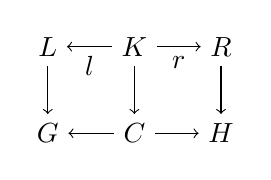
\begin{tikzpicture}[node distance=11mm]
          \node (I) {$K$};
          \node (L) [left of= I] {$L$};
          \node (R) [right of=I] {$R$}; 
          \node (G) [below of=L] {$G$};
          \node (C) [below of=I] {$C$};
          \node (H) [below of=R] {$H$};
        %   \node (T) [left=of $(L)!0.5!(G)$] {$T$};
        %   \draw [->] (L) to  node [label, above] {$c$}  (T);
        %   \draw [->] (G) to  node [label, below] {$\alpha$} (T);
          \draw [->] (I) to node [label, below] {$l$} (L);
          \draw [->] (I) to node [label, below] {$r$} (R);
          \draw [->] (L) to  (G);
          \draw [->] (I) to (C);
          \draw [->] (R) to (H);
          \draw [->] (C) to (G);
          \draw [->] (C) to (H);
        \end{tikzpicture}
      \end{center}
\end{minipage}
   \begin{itemize}
       \item $\operatorname{left}(\Delta)$ is weighable with \(\mathcal{T}\), and
       \item $\operatorname{right}(\Delta)$ is bounded above by \(\mathcal{T}\), and
       \item $w(e) \succeq 1_S$ for all $e \in \mathbb{E}$.
   \end{itemize}

   \noindent
  We have:
   \begin{itemize}
       \item $w_\mathcal{T}(G) \succeq w_\mathcal{T}(H)$ if $\rho$ is weakly decreasing, and
       \item $\mu(w_\mathcal{T}(G)) > \mu(w_\mathcal{T}(H)) + \delta$ if $\rho$ is $\delta$-uniformly or $\delta$-closure decreasing for some $\delta >0$, and $w(e) \succeq 1_S$ for all $e \in \mathbb{E}$.
   \end{itemize}
\end{lemma} 
\begin{proof}
   See the \hyperref[proof:decreasing_step]{Appendix}.
\end{proof}